\documentclass[12pt, twoside]{article}
\usepackage[letterpaper, margin=1in, headsep=0.5in]{geometry}
\usepackage[english]{babel}
\usepackage[utf8]{inputenc}
\usepackage{amsmath}
\usepackage{amsfonts}
\usepackage{amssymb}
\usepackage{tikz}
%\usetikzlibrary{quotes, angles}

\usepackage{graphicx}
\usepackage{enumitem}
\usepackage{multicol}

\usepackage{fancyhdr}
\pagestyle{fancy}
\fancyhf{}
\renewcommand{\headrulewidth}{0pt} % disable the underline of the header

\fancyhead[RE]{\thepage}
\fancyhead[RO]{\thepage \\ Name: \hspace{3cm}}
\fancyhead[L]{BECA / Dr. Huson / 10th Grade Geometry\\* 7 June 2019}

\begin{document}
\subsubsection*{Do Now: Angle relationships}
Find the section in your notebook with the theorems and formulas applying to these angle problems.
 \begin{enumerate}

 \item Given two vertical angles as shown, $m \angle 1 = 5x+5$, $m \angle 2 = 7x-17$.\\[0.5cm]
 Find $m \angle 1$.\\[0.5cm] For full credit find the $m\angle 2$ as a check.
   \begin{flushright}
   \begin{tikzpicture}[scale=.7]
     \draw [<->, thick] (0,-1.5)--(10,1.5);
     \draw [<->, thick] (2,3.5)--(7,-3.5);
     \node at (3,.4){1};
     \node at (6,-.6){2};
     %\draw [fill] (0,0) circle [radius=0.05] node[below]{$P$};
     %\draw [fill] (6,0) circle [radius=0.05] node[below]{$R$};
     %\draw [fill] (3,0) circle [radius=0.05] node[below]{$Q$};
   \end{tikzpicture}
   \end{flushright}
 \vspace{3cm}


 \item Given $\overrightarrow{BA} \perp \overrightarrow{BC}$, $m \angle ABD = 5x+47$, and $m \angle DBC = 2x+22$. Find $m \angle DBC$. \\[0.5cm]
 For full credit, show the check using both angle measures.
 \begin{flushleft}
 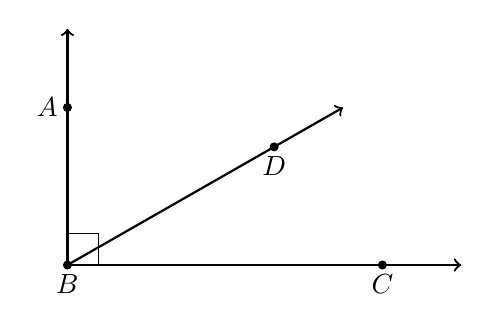
\begin{tikzpicture}[scale=1]
   \draw [<->, thick] (0,3)--(0,0)--(5,0);
   \draw [->, thick] (0,0)--(3.5, 2);
   \draw [-, thin] (0, 0.4)--(0.4, 0.4)--(0.4, 0);
   %\node at (3,.4){1};
   %\node at (6,-.6){2};
   \draw [fill] (0,0) circle [radius=0.05] node[below]{$B$};
   \draw [fill] (0,2) circle [radius=0.05] node[left]{$A$};
   \draw [fill] (4,0) circle [radius=0.05] node[below]{$C$};
   \draw [fill] (2.625, 1.5) circle [radius=0.05] node[below]{$D$};
 \end{tikzpicture}
 \end{flushleft}

 \newpage

  \item Given  $\triangle EFG$ with $\overline{EF}$ extended to $A$. If $m\angle F=40^\circ$ and $m\angle AEG=130^\circ$, what is $m\angle EGF$?
    \begin{center}
      \begin{tikzpicture}%[scale=0.7]
        \draw [thick](0,0)node[below]{$A$}--
          (2,0)node[below]{$E$}--
          (8,0)node[below]{$F$}--
          (4,3)node[above]{$G$} --(2,0);
      \end{tikzpicture}
    \end{center} %\vspace{4cm}

  \item Given $m\angle R=53^\circ$ and $m\angle UST=117^\circ$. Find $m\angle U$.\\[1cm]
    \begin{tikzpicture}
      %\draw [->, thick] (0,0)--(5,5);
      \draw [<-, thick] (8,0)--(0,0)--(3,3)--(4.5,0);
      \draw [fill] (0,0) circle [radius=0.05] node[below]{$R$};
      \draw [fill] (4.5,0) circle [radius=0.05] node[below]{$S$};
      \draw [fill] (3,3) circle [radius=0.05] node[right]{$U$};
      \draw [fill] (7,0) circle [radius=0.05] node[below]{$T$};
    \end{tikzpicture}
    \vspace{2cm}

  \item In  $\triangle ABC$ shown below, side $\overline{AC}$ is extended to point $D$ with $m\angle DAB=(180-2x)^\circ$, $m\angle C=(x-10)^\circ$, and $m\angle B=(3x+10)^\circ$.
    \begin{center}
      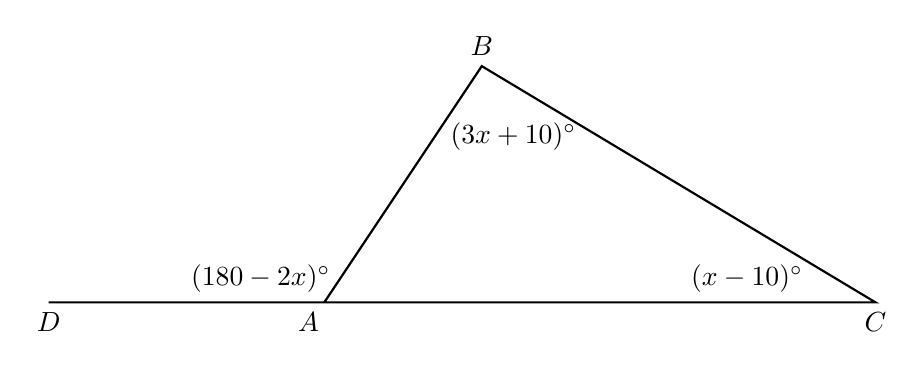
\begin{tikzpicture}
        \draw [thick](-1.5,0)node[below]{$D$}--
          (1.8,0)node[below]{$A$}--
          (9,0)node[below]{$C$}--
          (4,3)node[above]{$B$} --(2,0);
          \node at (2.2,0)[above left]{$(180-2x)^\circ$};
          \node at (8.2,0)[above left]{$(x-10)^\circ$};
          \node at (4.4,2.4)[below]{$(3x+10)^\circ$};
      \end{tikzpicture}
    \end{center}
    What is $m\angle BAC$?

\newpage

\item In  $\triangle ABC$ shown below, $m\angle A=(3x+4)^\circ$, $m\angle B=(5x-15)^\circ$, and $m\angle C=(x-7)^\circ$. What is $m\angle A$?\\[0.5cm]
    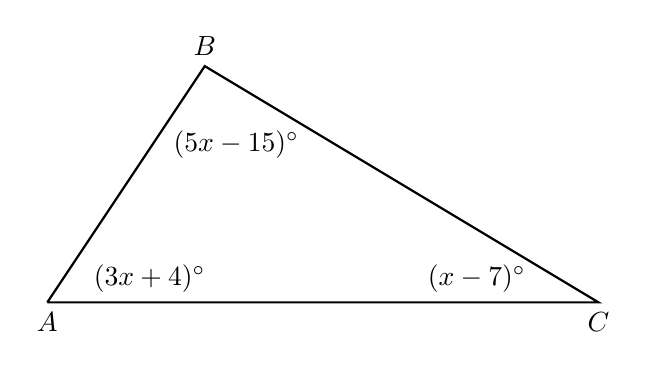
\begin{tikzpicture}
      \draw [thick]
        (2,0)node[below]{$A$}--
        (9,0)node[below]{$C$}--
        (4,3)node[above]{$B$} --(2,0);
        \node at (3.3,0)[above]{$(3x+4)^\circ$};
        \node at (8.2,0)[above left]{$(x-7)^\circ$};
        \node at (4.4,2.3)[below]{$(5x-15)^\circ$};
    \end{tikzpicture} \vspace{4cm}

\newpage

\item Given two parallel lines and a transversal, as shown below.
  \begin{center}
  \begin{tikzpicture}
    \draw [<->, thick] (1,2)--(9,2);
    \draw [<->, thick] (0,0)--(8,0);
    \draw [<->, thick] (4,-1)--(5.5,3);
    \node at (4.5,0.3) [left]{$5$};
    \node at (4.5,0.3) [right]{$6$};
    \node at (4.3,-0.3) [left]{$7$};
    \node at (4.3,-0.3) [right]{$8$};
    \node at (5.2,2) [above left]{$1$};
    \node at (5.2,2) [above right]{$2$};
    \node at (5,2) [below left]{$3$};
    \node at (5,2) [below right]{$4$};
  \end{tikzpicture}
  \end{center}
  \begin{enumerate}
    \item State the angle corresponding with $\angle 5$. \vspace{1cm}
    \item Given $m\angle 3 = 78^\circ$ and $m\angle 5 = 3x^\circ$. Find $x$. \vspace{3.5cm}
    \item In a proof, what reason would justify $\angle 3 \cong \angle 6$? \rule{6cm}{0.15mm}
  \end{enumerate}

  \item Given two parallel lines that intersect a transversal,  $\overleftrightarrow{DE} || \overleftrightarrow{BC}$. $m\angle ABC =3x-8$ and $m\angle BDE=6x+8$. \\[0.5]
  Find $m\angle ADE$.\\[2cm]
   \begin{tikzpicture}[scale=1.1]
     \draw [<->, thick] (-1,0)--(0,0)--(4,0);
     \draw [<->, thick] (-0.5,-0.5)--(3,3)--(3.5,3.5);
     \draw [<->, thick] (1,2)--(5, 2)--(5.5,2);
     \draw [fill] (3,3) circle [radius=0.05] node[above left]{$A$};
     \draw [fill] (5, 2) circle [radius=0.05] node[below]{$E$};
     \draw [fill] (2,2) circle [radius=0.05] node[above left]{$D$};
     \draw [fill] (0,0) circle [radius=0.05] node[above left]{$B$};
     \draw [fill] (3,0) circle [radius=0.05] node[below]{$C$};
   \end{tikzpicture} \vspace{4cm}

\newpage

\item Given $\triangle ABC$ and $\triangle DEC$ with $\angle B \cong \angle E$. $C$ is the midpoint of $\overline{BE}$.\\ Prove $\triangle ABC \cong \triangle DEC$.\\[0.5cm]
   \begin{tikzpicture}
       \draw [thick]
         (-1,2)node[right]{$B$}--
         (1,-2)node[left]{$E$}--
         (4,0)node[right]{$D$}--
         (0,0)node[below left]{$C$}--
         (-4,0)node[left]{$A$}--cycle;
     \end{tikzpicture}

   \begin{multicols}{2}
     \underline{Statement} \\
     \underline{Reason}
   \end{multicols}
   \begin{multicols}{2}
     \raggedcolumns
     \begin{enumerate}[label={\arabic*)}]
       \item \rule{4cm}{0.15mm} \vspace{0.3cm}
       \item \rule{4cm}{0.15mm} \vspace{0.3cm}
       \item \rule{4cm}{0.15mm} \vspace{0.3cm}
       \item $\angle BCA \cong \angle ECD$  \vspace{0.3cm}
       \item \rule{4cm}{0.15mm} \vspace{0.3cm}
       \item $\triangle ABC \cong \triangle DEC$ \vspace{0.3cm}
     \end{enumerate}
     \begin{enumerate}[label={\arabic*)}]
       \item Given \vspace{0.3cm}
       \item Given \vspace{0.3cm}
       \item Given \vspace{0.3cm}
       \item \rule{4cm}{0.15mm} \vspace{0.3cm}
       \item Definition of a midpoint \vspace{0.3cm}
       \item \rule{4cm}{0.15mm} \vspace{0.3cm}
     \end{enumerate}
   \end{multicols} %\vspace{0.5cm}


\end{enumerate}
\end{document}
